\documentclass[12pt]{article}
\usepackage[12pt]{moresize}
\usepackage[margin=1in]{geometry}

\usepackage{amsmath}
\usepackage{amssymb}

\usepackage{graphicx}
\usepackage{subcaption}

\usepackage{multirow} %Combining rows in tables
\usepackage{diagbox}  %Table box split in twain

\usepackage{algorithm}
\usepackage{algpseudocode}
\usepackage{alltt}

\usepackage{multicol}

\usepackage{amssymb} %\checkmark symbol

%\usepackage{hyperref}
%\usepackage[latin1]{inputenc}
%\usepackage{listings}
%\usepackage{scrextend}
%\usepackage{changepage} %Adjustwidth

 

\title{ComS 474\\Homework 6}
\author{Sean Gordon}
\date{Nov 19, 2020}

\begin{document}
\maketitle



\noindent 9) $W^{(0)}: 3\times3$, \ $W^{(1)}: 4\times2$, \ $W^{(2)}: 3\times2$\\



\noindent \hrulefill \\



\noindent 10) $x^1 = \phi\left[
\begin{pmatrix}
0.1 & 0.1 & 0.1\\
0.1 & 0.1 & 0.1\\
0.1 & 0.1 & 0.1
\end{pmatrix}
\begin{pmatrix}
1\\ 1\\ 1
\end{pmatrix}\right]=
\begin{pmatrix}
0.3\\ 0.3\\ 0.3
\end{pmatrix}$\\\\

\indent $x^2 = \phi\left[
\begin{pmatrix}
2 & 2 & 2 & 2\\
2 & 2 & 2 & 2
\end{pmatrix}
\begin{pmatrix}
1\\ 0.3\\ 0.3 \\ 0.3
\end{pmatrix}\right]=
\begin{pmatrix}
3.8\\ 3.8
\end{pmatrix}$\\\\

\indent $x^3 = \phi\left[
\begin{pmatrix}
1 & 1 & 1\\
1 & 1 & 1
\end{pmatrix}
\begin{pmatrix}
1\\ 3.8\\ 3.8
\end{pmatrix}\right]=
\begin{pmatrix}
8.6 \\ 8.6
\end{pmatrix}$\\\\



\noindent \hrulefill \\



\noindent 11) $\delta^{(3)} = 
\begin{pmatrix}
8.6 \\ 8.6
\end{pmatrix} - 
\begin{pmatrix}
1 \\ 0
\end{pmatrix} = 
\begin{pmatrix}
7.6 \\ 8.6
\end{pmatrix}$\\\\

\indent $\delta^{(2)} = 
\begin{pmatrix}
0(1 - 0) \\ 3.8(1 - 3.8) \\ 3.8(1 - 3.8)
\end{pmatrix} \circ \left(
\begin{pmatrix}
1 & 1 \\
1 & 1 \\
1 & 1 
\end{pmatrix}
\begin{pmatrix}
7.6 \\ 8.6
\end{pmatrix} \right) = 
\begin{pmatrix}
0 \\ -172.368 \\ -172.368
\end{pmatrix}
$\\\\

\indent $\delta^{(1)} = 
\begin{pmatrix}
0(1 - 0) \\ 0.3(1 - 0.3) \\ 0.3(1 - 0.3) \\ 0.3(1 - 0.3)
\end{pmatrix} \circ \left(
\begin{pmatrix}
2 & 2 \\
2 & 2 \\
2 & 2 \\
2 & 2 
\end{pmatrix}
\begin{pmatrix}
-172.368 \\ -172.368
\end{pmatrix}\right) = 
\begin{pmatrix}
0 \\ -144.789 \\ -144.789 \\ -144.789
\end{pmatrix}
$\\



\noindent \hrulefill \\\pagebreak



\noindent 12) $\nabla^{(2)} = x^{(2)}(\delta^{(3)})^T = 
\begin{pmatrix}
1\\ 3.8\\ 3.8
\end{pmatrix}
[7.6, 8.6] = 
\begin{pmatrix}
7.6 & 8.6 \\
28.88 & 32.68 \\
28.88 & 32.68
\end{pmatrix}
$\\\\

\indent $\nabla^{(1)} = x^{(1)}(\delta^{(2)})^T = 
\begin{pmatrix}
1\\ 0.3\\ 0.3 \\ 0.3
\end{pmatrix}
[-172.368, -172.368] = 
\begin{pmatrix}
-172.368 & -172.368 \\
-51.71 & -51.71 \\
-51.71 & -51.71 \\
-51.71 & -51.71 
\end{pmatrix}
$\\\\

\indent $\nabla^{(0)} = x^{(0)}(\delta^{(1)})^T = 
\begin{pmatrix}
1\\ 1\\ 1
\end{pmatrix}
[-144.789, -144.789, -144.789] = 
\begin{pmatrix}
-144.789 & -144.789 & -144.789 \\
-144.789 & -144.789 & -144.789 \\
-144.789 & -144.789 & -144.789 
\end{pmatrix}
$\\



\noindent \hrulefill \\



\noindent 13) $\mathbb{W}^{2} \leftarrow \mathbb{W}^{2} - \rho\nabla^{(2)} = 
\begin{pmatrix}
1 & 1 \\
1 & 1 \\
1 & 1 
\end{pmatrix} - 
\begin{pmatrix}
7.6 & 8.6 \\
28.88 & 32.68 \\
28.88 & 32.68
\end{pmatrix} = 
\begin{pmatrix}
-6.6 & -7.6 \\
-27.88 & -31.68 \\
-27.88 & -31.68
\end{pmatrix}
$\\\\

\indent $\mathbb{W}^{1} \leftarrow \mathbb{W}^{1} - \rho\nabla^{(1)} = 
\begin{pmatrix}
2 & 2 \\
2 & 2 \\
2 & 2 \\
2 & 2 
\end{pmatrix} - 
\begin{pmatrix}
-172.368 & -172.368 \\
-51.71 & -51.71 \\
-51.71 & -51.71 \\
-51.71 & -51.71 
\end{pmatrix} = 
\begin{pmatrix}
174.368 & 174.368 \\
53.71 & 53.71 \\
53.71 & 53.71 \\
53.71 & 53.71 
\end{pmatrix}
$\\\\

\indent $\mathbb{W}^{0} \leftarrow \mathbb{W}^{0} - \rho\nabla^{(0)} = 
\begin{pmatrix}
0.1 & 0.1 & 0.1\\
0.1 & 0.1 & 0.1\\
0.1 & 0.1 & 0.1
\end{pmatrix} - 
\begin{pmatrix}
-144.789 & -144.789 & -144.789 \\
-144.789 & -144.789 & -144.789 \\
-144.789 & -144.789 & -144.789 
\end{pmatrix} = $\\
\begin{center}$
\begin{pmatrix}
144.889 & 144.889 & 144.889 \\
144.889 & 144.889 & 144.889 \\
144.889 & 144.889 & 144.889 
\end{pmatrix}$
\end{center}


\noindent \hrulefill \\




%\begin{figure}[htbp]
%\centerline{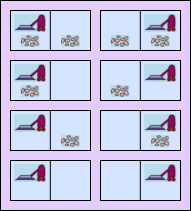
\includegraphics{Pics/ComS472_410.png}}
%\caption{Belief states recheable from initial 8 belief states.}
%\label{Belief states recheable from initial 8 belief states.}
%\end{figure}

\end{document}

















